\documentclass[11pt]{article}

\usepackage[margin=1in]{geometry}
\usepackage[T1]{fontenc}
\usepackage{amsmath, amssymb}
\usepackage{graphicx}
\usepackage{booktabs}
\usepackage{caption}
\usepackage{listings}
\usepackage{xcolor}
\usepackage[colorlinks=true, allcolors=blue!60!black]{hyperref}

\graphicspath{{figures/}}

% Placeholder marker. Delete every one of these before submitting.
\newcommand{\tbd}[1]{\textcolor{red}{[#1]}}

% LENGTH: limit is 3-5 pages, appendix excluded. Check the page count first
% thing on Overleaf. If it is over, cut in this order:
%   1. Section 5, the "distinction the model cannot see" paragraph (interesting,
%      not required by either research question)
%   2. Section 5, the Robustness paragraph (one sentence would do)
%   3. Section 2, the Measurement paragraph (compress to two sentences)
%   4. Figure 2 to the appendix, leaving Figure 1 as the only results figure

\lstset{
  basicstyle=\ttfamily\footnotesize,
  keywordstyle=\color{blue!60!black},
  commentstyle=\color{gray},
  stringstyle=\color{green!40!black},
  breaklines=true,
  frame=single,
  rulecolor=\color{gray!40},
  language=Python,
  showstringspaces=false
}

\title{Modeling Student Priorities: Using Linear Algebra to Approximate the
True Significance of Workload vs.\ Professor Quality to Yale Students Across
the Disciplines}
\author{\tbd{Member A} \and \tbd{Member B} \and Selinam Mortey}
\date{\today}

\begin{document}
\maketitle

\section{Introduction}

\tbd{0.5 page. Course selection at Yale; what OCE and CourseTable are and how
students actually use them; why the trade-off between workload and teaching
quality is the interesting one.}

This project asks two questions.

\begin{quote}
\textbf{Q1.} How much do workload and teaching quality each contribute to a
course's overall rating in STEM, Humanities and Social Science courses at Yale,
and does CourseTable's summary data tell the same story as the raw evaluations?

\textbf{Q2.} Which courses are ``hidden gems'' --- meaning their overall rating
is far above what the model predicts from workload and teaching quality --- and
where do they occur?
\end{quote}

Throughout we speak about \emph{courses}, not \emph{students} or \emph{majors}:
the unit of observation is one course's set of evaluation averages, so the data
cannot support a claim about what any individual student wants.

\section{Data}

\textbf{Sources.} Yale Online Course Evaluations (OCE), viewed through Yale
Course Search, supply five question averages per course: Q4 overall assessment
($y$), Q5 ``well organized'', Q6 ``clear feedback'', Q7 intellectual challenge,
and Q8 workload relative to other Yale courses ($x_1$). Teaching quality $x_2$
is the mean of Q5 and Q6. CourseTable, the student-run catalogue maintained by
the Yale Computer Society, supplies a course rating, a professor rating and a
workload figure for the same courses, taken from its published Fall 2025 export.

One property of that export matters for the whole comparison: its figures are
averaged across \emph{past offerings} of a course, not computed from the term in
question. 287 courses with no Fall 2025 responses at all still carry a rating.
Model~B is therefore not a second measurement of the same thing --- it is the
prior reputation a student consults before enrolling, set against what that
term's students went on to report.

\textbf{Term and sampling.} Fall 2025. Courses were assigned to a discipline by
Yale's own distributional area tags --- \texttt{Hu}, \texttt{So}, \texttt{Sc}
--- rather than by a classification of our own, which removes a judgment call
from the design. Mathematics and computer science carry no area tag, since Yale
files them under the quantitative-reasoning \emph{skill}, so untagged courses
whose first-listed subject is MATH, CPSC, S\&DS, AMTH or ENAS were added to the
sciences; the skill tag alone is no use as a marker, because 96 economics
courses also carry it. Courses with two or more area tags were excluded as
ambiguous.

The eligible frame is every Yale College course that term with one area, at
least 8 responses and complete CourseTable figures: 223 humanities, 140 social
science, 195 science. From each, 25 courses were drawn with a fixed random seed.
Every sampled course had a published evaluation, so the analysis uses all 75.
Because only about 40\% of eligible courses carry a CourseTable professor
rating, the draw was restricted to those that do, so both models are fitted on
identical courses; the sample therefore represents courses CourseTable holds
professor data for, not all Yale courses.

\textbf{Measurement.} OCE publishes each average rounded to one decimal place.
Rather than use those figures we recorded the individual responses behind them
and computed each mean exactly as $\bar q = \sum_k k\,c_k / \sum_k c_k$. At
$n = 25$ the rounding would otherwise add roughly $\pm 0.05$ of noise to every
variable, attenuating the correlations being estimated. It also gives the
correct $n$ per question, which is not the course's response count: students
skip questions.

\textbf{Quality control.} Three checks. Each of the 375 computed means was
compared against the figure OCE displays: the largest discrepancy was $0.0500$,
exactly the half-step of OCE's rounding, and none fell outside it. CourseTable's
response count was compared against OCE's: all 75 agreed exactly. Our area-tag
discipline was compared against OCE's own primary division, agreeing on 69 of
the 71 courses where OCE reports a comparable one; the exceptions, EVST 3255 and
NSCI 1600, are cross-listed courses whose department differs from the area the
course itself carries, and we keep the area tag.

\section{The linear algebra}

Write $A \in \mathbb{R}^{n \times 3}$ for the design matrix whose rows are
$\begin{bmatrix} 1 & x_{1i} & x_{2i}\end{bmatrix}$ and $y \in \mathbb{R}^n$ for
the vector of overall ratings. In general no $\beta$ satisfies $A\beta = y$
exactly, because $y$ almost never lies in the three-dimensional subspace
$\operatorname{Col}(A) \subset \mathbb{R}^n$. The least-squares problem is
therefore to find the $\hat\beta$ minimizing $\|y - A\beta\|$, which is the same
as finding the point of $\operatorname{Col}(A)$ closest to $y$.

That point is the orthogonal projection of $y$ onto $\operatorname{Col}(A)$. The
residual $e = y - A\hat\beta$ must be orthogonal to every column of $A$, which
is exactly the statement $A^{\mathsf T}e = 0$, and expanding it gives the normal
equations
\begin{equation}
  A^{\mathsf T}A\,\hat\beta = A^{\mathsf T}y .
\end{equation}
When the columns of $A$ are linearly independent, $A^{\mathsf T}A$ is invertible
and $\hat\beta = (A^{\mathsf T}A)^{-1}A^{\mathsf T}y$ is unique, with fitted
values $\hat y = Py$ for the projection matrix
$P = A(A^{\mathsf T}A)^{-1}A^{\mathsf T}$. Independence holds here as long as
workload and teaching quality are not perfectly correlated across the sampled
courses, which we check directly.

\begin{figure}[h]
  \centering
  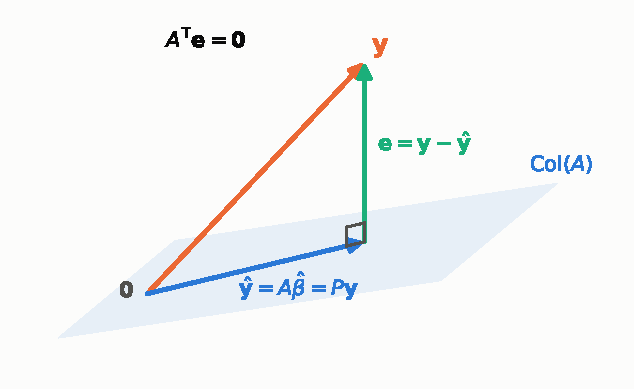
\includegraphics[width=0.48\textwidth]{fig5_projection}
  \caption{Least squares as projection: $\hat y$ is the closest point of
  $\operatorname{Col}(A)$ to $y$, and the residual leaves at a right angle, so
  $A^{\mathsf T}e = 0$.}
  \label{fig:projection}
\end{figure}

\textbf{SVD and conditioning.} Writing $A = U\Sigma V^{\mathsf T}$ gives the
equivalent solution $\hat\beta = V\Sigma^{+}U^{\mathsf T}y$ through the
pseudoinverse, which we compute as a check. The singular values also give the
condition number $\kappa(A) = \sigma_{\max}/\sigma_{\min}$. Because
$\kappa(A^{\mathsf T}A) = \kappa(A)^2$, forming the normal equations squares the
conditioning, which is the standard reason to prefer an SVD or QR route when the
predictors are strongly correlated. Our condition numbers run from $1.05$ to
$3.88$, so $\kappa(A^{\mathsf T}A)$ never exceeds about $15$ and the two routes
agree to machine precision.

\textbf{Goodness of fit.} We report $R^2 = 1 - \|e\|^2 / \|y - \bar y\|^2$, the
share of the variation in overall rating the two predictors account for.

\section{Applying it}

All three variables are standardized within each discipline before fitting, so
$\hat\beta_1$ and $\hat\beta_2$ are directly comparable: each is the change in
overall rating, in standard deviations, per one-standard-deviation change in its
predictor. Model~A uses the OCE figures; Model~B repeats the fit with
CourseTable's rating, workload and professor score on the same courses.

Uncertainty comes from a bootstrap: courses are resampled with replacement 1000
times within each discipline and the model refitted, giving a 95\% interval from
the 2.5th and 97.5th percentiles of each weight.

For hidden gems we fit one \emph{pooled} model across all 75 courses so
that every course is judged on the same scale, adding two discipline indicator
columns. Only two are included: a third, alongside the intercept column, would
make the columns of $A$ linearly dependent and $A^{\mathsf T}A$ singular. STEM
is the omitted baseline. A course is flagged when its standardized residual
$r_i = e_i / s$, with $s = \sqrt{\|e\|^2/(n-p)}$, exceeds 2.

The computation was done in Python with NumPy for the matrix algebra, pandas for
the data handling and matplotlib for the figures; $\hat\beta$ is obtained from
the normal equations with \texttt{np.linalg.solve}, and
\texttt{np.linalg.lstsq}, the SVD route and \texttt{statsmodels} OLS are used
only to confirm it. The core routine is in the appendix.

\section{Results}

\textbf{Q1a and Q1b: what carries a course's rating.} Table~\ref{tab:betas} and
Figure~\ref{fig:weights} give the standardized weights. The result is the same
in all three disciplines and is not subtle. Instructional quality carries almost
the entire fit: $\hat\beta_{\text{teaching}} = 0.84$ in the humanities, $0.89$
in the social sciences and $0.94$ in STEM. Workload carries essentially nothing:
$-0.07$, $+0.08$ and $-0.05$ respectively, with the social-science estimate
pointing in the opposite direction to the one usually assumed. The model
accounts for $R^2 = 0.69$, $0.79$ and $0.86$ of the variation in overall rating.

Bootstrap intervals (Table~\ref{tab:ci}, and the error bars in
Figure~\ref{fig:weights}) settle whether this is noise. All three teaching
intervals sit clear of zero; all three workload intervals contain it ---
$[-0.25, 0.19]$, $[-0.14, 0.24]$, $[-0.18, 0.12]$. The predictors are nearly
uncorrelated within discipline ($r = 0.16$, $-0.05$, $0.32$), so this is not
collinearity hiding a workload effect behind teaching quality: the columns of
$A$ are close to orthogonal and workload still explains nothing.

\textbf{A distinction the model cannot see.} This concerns variation
\emph{within} a discipline, since every variable is standardized within
discipline before fitting. Between disciplines the picture differs: mean
workload rises across humanities, social sciences and STEM ($2.86$, $3.10$,
$3.32$) while mean rating falls ($4.33$, $4.13$, $3.80$). Our design removes
that variation deliberately, and with three disciplines it could not be tested
anyway --- the ordering is equally consistent with differing grading cultures or
student populations. The claim we can defend is narrow: among courses competing
within one discipline, how hard a course is tells you nothing about how highly
it is rated.

\textbf{Q1c: does CourseTable agree?} Fitting the same model to its figures
(Table~\ref{tab:compare}) gives the same shape --- the professor rating carries
it ($0.75$, $0.66$, $0.53$, all clear of zero), workload contributes nothing ---
and its measures track the evaluations closely ($r = 0.91$ for workload, $0.83$
for the course rating). But explanatory power is markedly \emph{lower}:
$R^2 = 0.55$, $0.43$, $0.28$ against $0.69$, $0.79$, $0.86$. We expected the
opposite. The cause is scope: CourseTable averages across past offerings, so it
describes reputation rather than the term measured, and that mismatch costs
accuracy.

Figure~\ref{fig:circularity} (appendix) tests whether its professor rating is
really the course rating relabelled. It correlates $0.66$ with the overall-course question
and $0.60$ with the teaching questions. The gap leans the way the circularity
hypothesis predicts but is too small to support it; the professor rating looks
like a genuinely distinct instructor-level measurement, noisier here only
because it is not term-specific.

\textbf{Q2: hidden gems.} No course reached a standardized residual above $2$,
so under D8 we report the top $5\%$ (Table~\ref{tab:gems}): SOCY 2009
($r_i = 1.79$), ECON 4444 ($1.67$), MUSI 2240 ($1.66$), CPSC 4670 ($1.64$).
That the threshold caught nothing is itself the finding --- a model explaining
69--86\% of the variance leaves little room for a course to sit far above its
prediction, so the hidden gem is close to nonexistent. The breakdown by class
size (Figure~\ref{fig:gemrate}, appendix) has cells far too thin to support a
conclusion and we draw none. The same rule on CourseTable's figures flags three
courses --- PLSC 3511, PHYS 0700, MCDB 4820 --- sharing \emph{no} members with
the OCE list.

\textbf{Robustness.} Adding Q7 changes nothing: teaching stays at $0.84$,
$0.88$, $0.93$, workload stays indistinguishable from zero, challenge
contributes little ($0.04$, $0.13$, $0.08$), and $R^2$ moves by under $0.01$
everywhere. $\kappa(A)$ rises from about $1.2$ to $2.4$--$3.9$ with the third
column, still far from troublesome.

\begin{figure}[h]
  \centering
  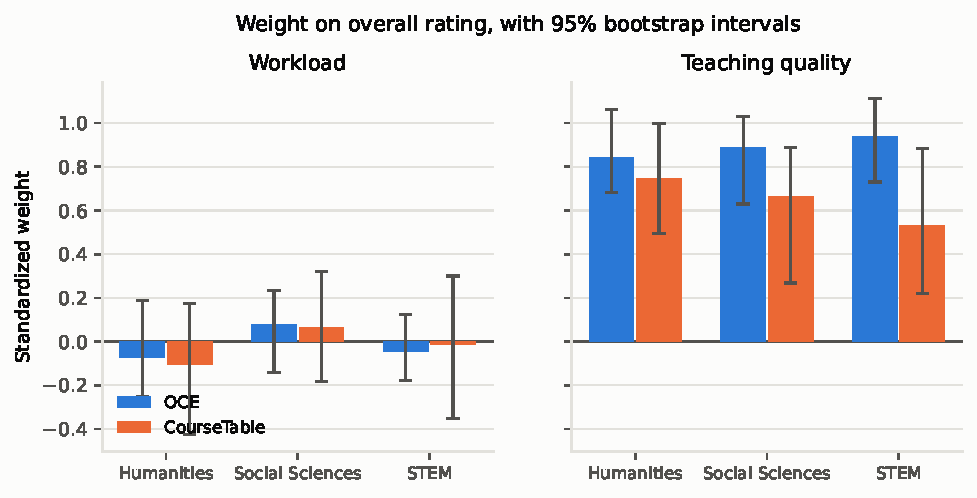
\includegraphics[width=0.88\textwidth]{fig1_weights}
  \caption{Standardized weights on overall rating by discipline, with 95\%
  bootstrap intervals, for the evaluation data and for CourseTable's summary
  figures.}
  \label{fig:weights}
\end{figure}

\begin{table}[h]
  \centering
  \caption{Standardized least-squares weights from the evaluation data, by discipline.}
  \label{tab:betas}
\begin{tabular}{lrrrrrr}
\toprule
Discipline & $n$ & $\hat\beta_{\text{workload}}$ & $\hat\beta_{\text{teaching}}$ & $R^2$ & $r(x_1,x_2)$ & $\kappa(A)$ \\
\midrule
Humanities & 25 & -0.07 & 0.84 & 0.69 & 0.16 & 1.18 \\
Social Sciences & 25 & 0.08 & 0.89 & 0.79 & -0.05 & 1.05 \\
STEM & 25 & -0.05 & 0.94 & 0.86 & 0.32 & 1.39 \\
\bottomrule
\end{tabular}
\end{table}


\begin{figure}[h]
  \centering
  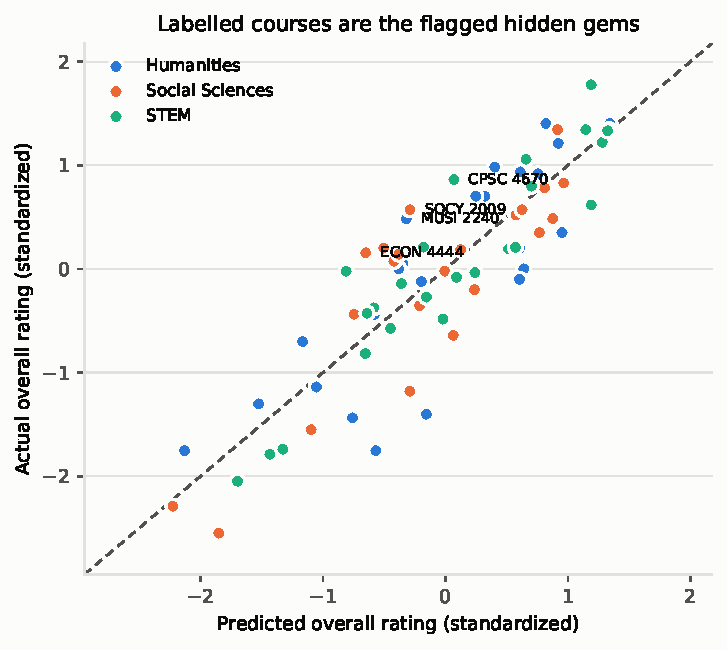
\includegraphics[width=0.5\textwidth]{fig2_actual_vs_predicted}
  \caption{Actual against predicted overall rating. Labelled points are the
  flagged hidden gems.}
  \label{fig:gems}
\end{figure}

\textbf{Numerical checks.} Across every fit, $\max|A^{\mathsf T}e| <
8 \times 10^{-15}$, confirming numerically that the residual is orthogonal to
the column space, and the normal-equation solution agreed with the SVD,
\texttt{np.linalg.lstsq} and \texttt{statsmodels} solutions to within
\texttt{np.allclose} tolerance in every case.

\section{Discussion and limitations}

\textbf{The predictors and the response come from the same survey.} This is the
limitation that most constrains what the results mean, and it deserves stating
before any other. Overall assessment, organization and feedback are three items
on one form, answered by the same student in the same sitting. A student who
enjoyed a course tends to rate every item highly, so part of the $0.90$
correlation between instructional quality and overall rating reflects a shared
response disposition rather than teaching causing satisfaction. The high $R^2$
should be read as evidence that these items move together, not as evidence that
teaching quality determines a course's worth. Separating the two would need a
measure of teaching collected independently of the students doing the rating,
which no publicly available Yale source provides.

The remaining limitations are: one term only, so nothing here speaks to change
over time; course-level rather than student-level data, so no claim about
individual students or majors follows; response bias, since students who
complete evaluations are not a random subset of those enrolled; ordinal 1--5
scales treated as numeric and averaged; $n = 25$ per discipline, which the
bootstrap intervals reflect; a sample restricted to courses for which
CourseTable holds a professor rating; class size unevenly distributed across the
sample (40 seminars, 25 mid-sized, 10 lectures), so the size comparison in
Figure~\ref{fig:gemrate} rests on thin cells; and CourseTable's metrics being
derived quantities, averaged over past offerings, whose definitions we do not
control.

\section{Conclusion}

\textbf{Q1.} Within a discipline, a course's overall rating is carried almost
entirely by how well it is taught and essentially not at all by how much work it
demands: the standardized weight on instructional quality is $0.84$, $0.89$ and
$0.94$ across humanities, social sciences and STEM, every bootstrap interval
clear of zero, while the weight on workload is indistinguishable from zero in
all three. We expected the disciplines to differ and they did not. CourseTable
points the same way but fits less well ($R^2 = 0.28$--$0.55$ against
$0.69$--$0.86$) because it averages across past offerings, and its professor
rating tracks the overall question only slightly more closely than the teaching
questions ($0.66$ against $0.60$) --- too small a gap to call it the course
rating relabelled.

\textbf{Q2.} Hidden gems barely exist. No course exceeded a standardized
residual of $2$, and the top $5\%$ reach only $1.64$--$1.79$, because workload
and teaching quality already account for most of the variation. The same rule on
CourseTable's figures flags three entirely different courses.

One caveat governs all of it (Section~6): response and predictors are items on
the same survey, answered by the same student at the same moment. We have
measured that a student's judgement of teaching and of the course move together
closely while their report of workload moves independently of both --- a real
finding about course evaluations, but not evidence that better teaching causes a
better course.

\appendix
\section{Code}

\lstinputlisting[caption={Least squares by the normal equations, with the SVD
and library cross-checks (\texttt{src/model.py}).},
linerange={18-51}]{../src/model.py}

\lstinputlisting[caption={Hidden-gem rule (\texttt{src/gems.py}).},
linerange={17-45}]{../src/gems.py}

\section{Supporting tables and figures}

\begin{table}[h]
  \centering
  \caption{Courses flagged as hidden gems.}
  \label{tab:gems}
\begin{tabular}{lrrrrrr}
\toprule
Course & Discipline & Class size & Actual & Predicted (std.) & $r_i$ & Rule \\
\midrule
SOCY 2009 & Social Sciences & seminar & 4.50 & -0.29 & 1.79 & top 5\% \\
ECON 4444 & Social Sciences & mid & 4.23 & -0.65 & 1.67 & top 5\% \\
MUSI 2240 & Humanities & mid & 4.56 & -0.32 & 1.66 & top 5\% \\
CPSC 4670 & STEM & seminar & 4.33 & 0.07 & 1.64 & top 5\% \\
\bottomrule
\end{tabular}
\end{table}

\begin{table}[h]
  \centering
  \caption{Bootstrap 95\% intervals, 1000 resamples within each discipline.}
  \label{tab:ci}
\begin{tabular}{lrrrr}
\toprule
Discipline & Predictor & Estimate & 2.5\% & 97.5\% \\
\midrule
Humanities & workload & -0.07 & -0.25 & 0.19 \\
Humanities & teaching & 0.84 & 0.68 & 1.06 \\
Social Sciences & workload & 0.08 & -0.14 & 0.23 \\
Social Sciences & teaching & 0.89 & 0.63 & 1.03 \\
STEM & workload & -0.05 & -0.18 & 0.12 \\
STEM & teaching & 0.94 & 0.73 & 1.11 \\
\bottomrule
\end{tabular}
\end{table}

\begin{table}[h]
  \centering
  \caption{The same model fitted to the evaluation data and to CourseTable's summary figures.}
  \label{tab:compare}
\begin{tabular}{lrrrrrr}
\toprule
Discipline & Workload (OCE) & Teaching (OCE) & $R^2$ (OCE) & Workload (CT) & Professor (CT) & $R^2$ (CT) \\
\midrule
Humanities & -0.07 & 0.84 & 0.69 & -0.10 & 0.75 & 0.55 \\
Social Sciences & 0.08 & 0.89 & 0.79 & 0.06 & 0.66 & 0.43 \\
STEM & -0.05 & 0.94 & 0.86 & -0.01 & 0.53 & 0.28 \\
\bottomrule
\end{tabular}
\end{table}


\begin{figure}[h]
  \centering
  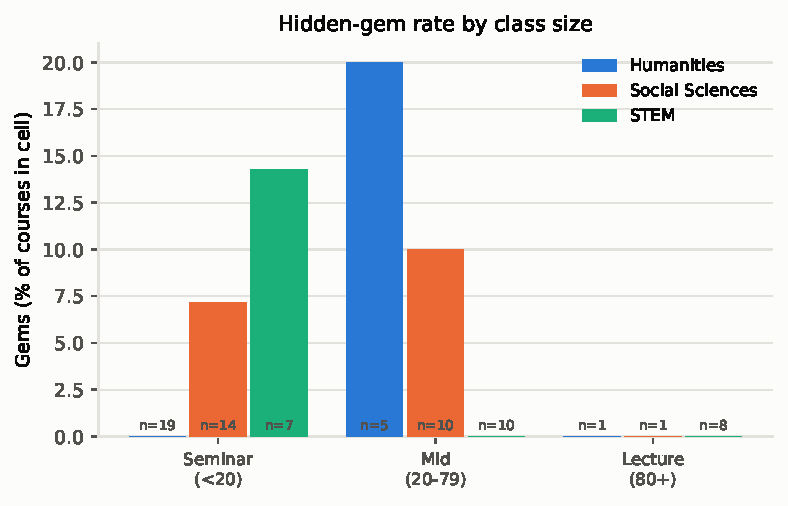
\includegraphics[width=0.72\textwidth]{fig3_gem_rate}
  \caption{Hidden-gem rate by class size and discipline. Reported for
  completeness; the cells are too thin to support a conclusion.}
  \label{fig:gemrate}
\end{figure}

\begin{figure}[h]
  \centering
  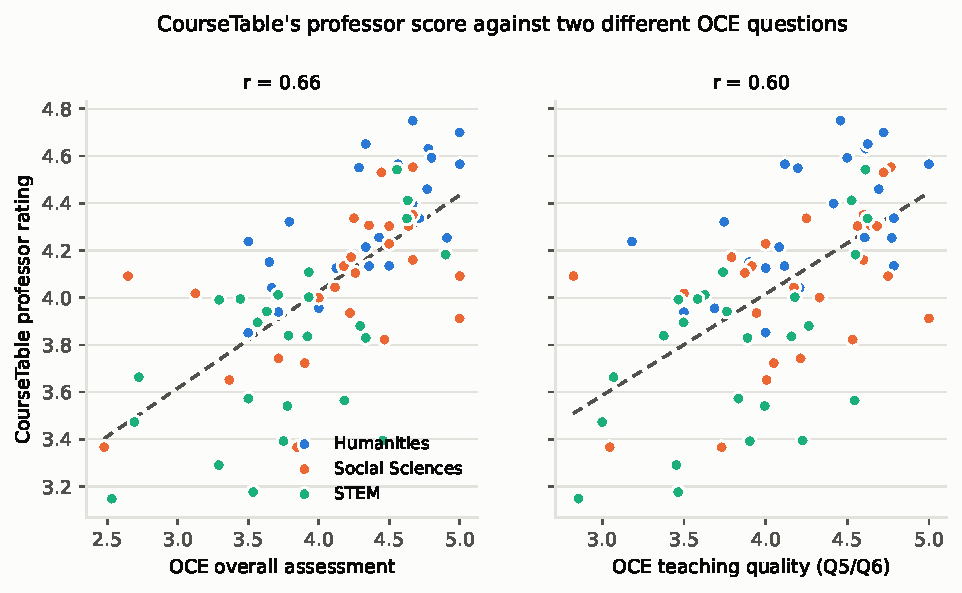
\includegraphics[width=0.92\textwidth]{fig4_circularity}
  \caption{CourseTable's professor rating against the OCE overall assessment and
  against the OCE teaching questions (the circularity test for Q1c).}
  \label{fig:circularity}
\end{figure}

\end{document}
